\documentclass[sigconf]{acmart}

\usepackage{graphicx}
\usepackage{hyperref}
\usepackage{todonotes}

\usepackage{endfloat}
\renewcommand{\efloatseparator}{\mbox{}} % no new page between figures

\usepackage{booktabs} % For formal tables

\settopmatter{printacmref=false} % Removes citation information below abstract
\renewcommand\footnotetextcopyrightpermission[1]{} % removes footnote with conference information in first column
\pagestyle{plain} % removes running headers

\newcommand{\TODO}[1]{\todo[inline]{#1}}

\begin{document}
\title{MQTT for Big Data and Edge Computing}


\author{Janaki Mudvari Khatiwada}
\orcid{1234-5678-9012}
\affiliation{%
  \institution{Indiana University, Bloomington}
  \streetaddress{P.O. Box 1212}
  \city{Bloomington} 
  \state{Indiana} 
  \postcode{43017-6221}
}
\email{jmudvari@iu.edu}





\begin{abstract}
With increasing use of sensors and smart devices or internet of things that generate real time data and opt for immediate output, immediate message delivery and reliable result is a must. This requires reliable efficient connection among sensors and near end devices. MQTT protocol  establishes the connection among participating clients. Traditionally connected  devices and industrial automation equipment are  connected to cloud. Data flow between cloud services and internet of things may not be reliable and efficient all the time. With growing number of smart devices, internet of things and their applications, communications between them and cloud services need reliable internet connection with no data limitations. Edge computing, data flow between near end devices, under MQTT can be a solution to improve latency of data flow,  better scalability and taking load off on local servers.
\end{abstract}

\keywords{i523, hid330, MQTT, Big Data, Edge Computing }


\maketitle



\section{Introduction}

MQTT, MQ telemetry transport protocol is an open source, a light--weight  reliable publish and subscribe messaging protocol on top op TCP/IP protocol. It's  use is intended for wireless and low band--width connection. It acts as a broker between clients or a server. Both publisher and subscriber are MQTT clients. It was invented in 1999 by Andy Stanford--Clark and Arlen Nipper. It was designed for communicating messages between clients in remote locations that had limited network bandwidth. We have come a long way since then  with all new sensors and smart devices and internet of things (IoTs) that are live streaming  data. These devices are connected to the cloud through sensors. Flow of data from cloud to these devices or vice--versa may be latent because of slower connectivity and depend upon the devices' performance. However, these internet of things require efficient flow of information in an instant. Reliable flow of these data among IoTs need reliable connection between server and its clients which may need higher band--with server. Servers should be able to convey messages subscribed by their clients within milliseconds. This is when edge computing comes into play. Edge computing is data analysis nearby these devices so that there is less load on the main server.  All clients or smart devices are connected to the broker and broker publish messages to each client based upon their subscription topic. Popular MQTT broker such as Mosquito, HiveMQ also support web sockets so that a web page of a modern web browser can connect to the MQTT broker and can subscribe on a topic and display real time data. MQTT supports transport layer security and authenticate with username  and password. Raspberry Pi, esp8266 are small devices or small computer that have built--in support for wireless LAN which can be employed as an edge device, after being integrated with MQTT,  for data transmission 

Why are we discussing Edge computing and MQTT? While MQTT was in use since 1999, it gained its significance recently. As with the development of IoTs and their newer applications, MQTT is seen as a light weight open source protocol that can establish a connection between server and its near end devices and help in quick message delivery. The number of connected devices are expected to reach 50 billion by 2020, from 500 million in 2003 to 12.5 billion in 2010. These sensors and devices generate huge volume of data and send to the cloud in a great velocity. This big data transmission to the cloud, which is a centralized data center, puts all the computation load on cloud and result in latent message transformation. Most of the applications in these smart devices need real time analysis and immediate message delivery on the topic they subscribe. Edge computing basically allows decentralization of data flow between these devices, servers and users. Further, edge computing significantly takes load off of cloud computing. Edge computing architecture facilitates data transmission between sensors and connected devices to a nearby edge computing device, ``like a gateway device that processes or analyzes the data locally, rather than sending it to the cloud or a remote data center'' \cite{www-rtinsights-com}. A gateway could be a server or a feature of the router or a computer that helps connect devices with the data--center network.
Figure\ref{p:Pub/Sub MQTT} below gives a general idea of message transmission through MQTT protoclo. In this figure HiveMQ is an open source MQTT broker. 

\begin{figure}[htb]
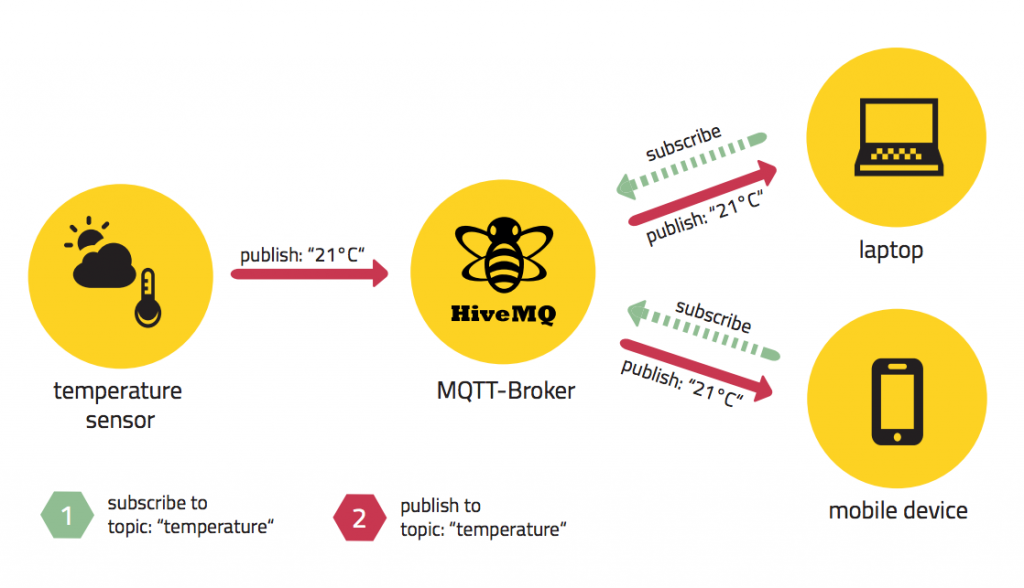
\includegraphics[width=1.0\columnwidth]{images/pubsubmqtt.png}
\caption{Pub/Sub MQTT}\label{p:Pub/Sub MQTT}
\end{figure}

\section{Applications}
A general mobile app such as facebook messenger that uses MQQT server for sending and receiving messages using MQQT library is a simple example of MQQT Application. This application runs on smart devices like smartphones and tablets.
Remote monitoring of manufacturing plants, smart grid, transportation, traffic monitoring, surveillance cameras,emergency response, industrial IoTs, smart home automation, Amazon Web Services, Facebook messenger are some of the notable  applications of MQTT protocol for edge computing. According to an estimate by Cisco, the amount of ``data generated by people, machines and things will be 600 zetta--bytes(ZB) which is up from 145 ZB generated in 2015'' \cite{www-rtinsights-com}. 

Industries can benefit by using MQQT protocol for edge computing since the devices and sensors may be located in remote locations. Remote locations might have network constraints such as lower connectivity, data limitations and and high latency. Given its lightweight feature MQTT protocol is ideal for data transmissions under such circumstances. Edge computing provides platform to the industries, social and government organizations so that they are able to analyze required data at the right location in the network in real time. By adopting their operations to the platform of edge computing industries could make use of these data not only to increase their profits but also enhance their operational efficiency. ``Ignition Industrial Internet of Things provides an MQQT architecture platform to industries and business applications'' \cite{inductiveautomation-com}. 

Monitoring patient at home is a good use case of application of MQTT protocol. Patient with implanted cardioverter defibrillator, which communicates with the hospital, can be monitored remotely along with the implanted device. Device's and patient's data are transmitted to the MQTT device located in patient's residence. Data is transmitted to the hospital by a transmitter that helps to analyze the condition of the patient. This helps to reduce hospital visits \cite{www-ibm-com/support}. It also detects emergency and notify on--call physician. The whole monitoring system is simple on patient's part as the device is already configured for MQQT client implementation by the the supplier or developer. Patient just needs to plug it in for power supply.

Another use case of MQQT protocol for big data and edge computing is environment monitoring for which sensors are most likely located in remote locations with intermittent network  connection. Environmental sensors depending on the topic such as water level sensor, need to constantly stream data from the location and others such as pollutant sensors store data in in their system and transfer them in a timely manner. Home automation is another  very good example of above discussed topic. Single broker or MQTT server establishes connection with smart devices around the house such as coffee--maker, air conditioner, lights, doors and others whenever required they are able to publish messages to the client upon subscription to the topic. The figure \ref{p:MQTT Architecture for Edge Computing} mentioned below sums of the MQTT for big data and edge computing.
\begin{figure}
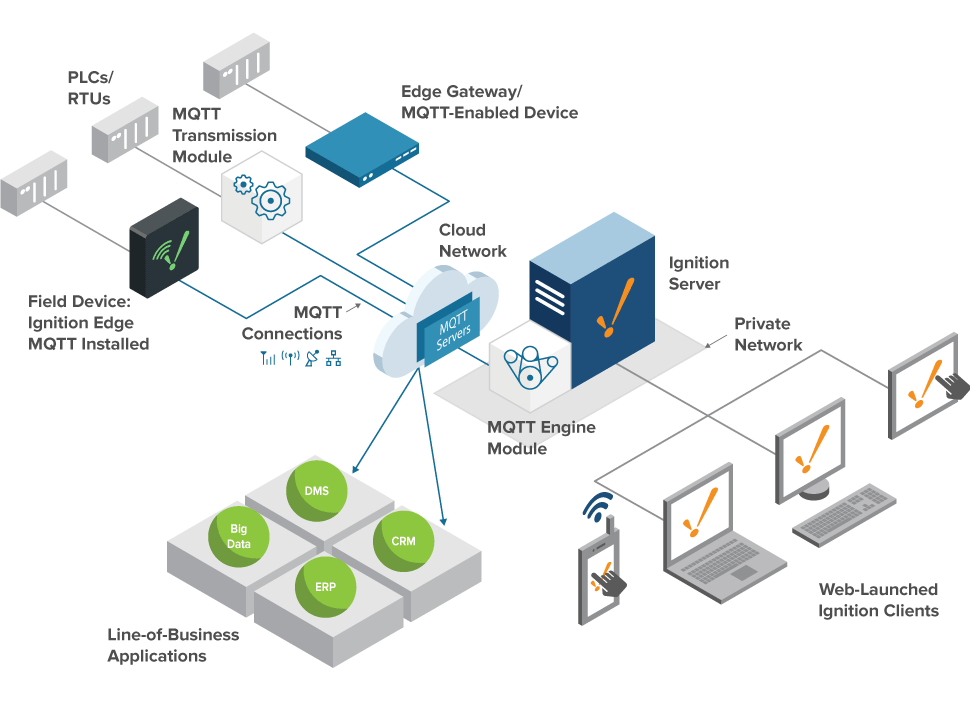
\includegraphics[width=1.0\columnwidth]{images/mqttArchitectureforEdgeComputing.png}
\caption{MQTT Architecture for Edge Computing}\label{p:MQTT Architecture for Edge Computing}


\end{figure}






\section{MQTT Work--Flow}
The work flow of MQTT starts by establishing connection of a broker, which is a local server, to a client. Clients are devices connected to a broker. There is at least one MQTT client responsible for publishing a message and second client which receives the message has to be subscribed to the topic in which first client is publishing a message. A message can be a data or command. Topic is a string separated by slashes. For example, ``home/kitchen/light1'' is a topic. Then client can also subscribe to a topic to a different device through a different command. MQTT client and server communicate through different control packets as shown in figure \ref{p:Publish Subscribe Architecture}.

\begin{figure}[htb]
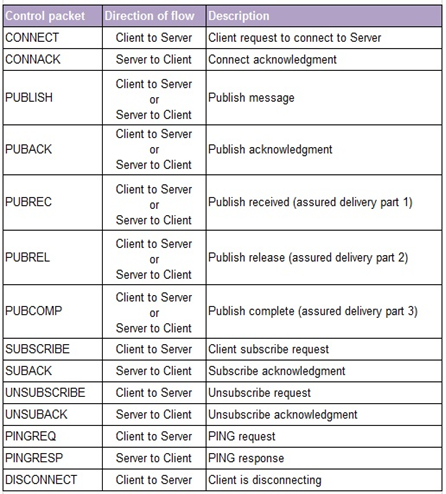
\includegraphics[width=1.0\columnwidth]{images/MQTT.png}
\caption{MQTT publish Subscribe Architecture}\label{p:Publish Subscribe Architecture}
\end{figure}


MQTT broker receives all the messages, filters them and publishes them to each subscribed clients. one of the important feature of this protocol is it decouples devices and applications before transmitting messages or data. Each MQTT message contains a topic, payload which may be in any format like binary data or plain text or xml. Quality of service is another feature of MQTT. It has three standard quality of services (QoS) for message delivery; 0, 1, 2. QoS 0 means message is delivered at most once, QoS 1 means message is delivered at least once, so duplicate message is possible and QoS 2 means message is delivered exactly once and there will be no duplicates but message is guaranteed.

For securing the data transmission both MQTT broker and clients authenticate each other by providing username and password during transmission and application level. Both broker and clients transmit acknowledgement message after connection, subscription and publishing of message. Another feature of MQTT is 'Last Will and Testament', which is used to notify other clients when a client is suddenly disconnected. Each client can specify its last will  as a message in certain topic with quality of service, message retained and payload features. Message specified in last will and testament will be send to all the clients upon disconnection of a client \cite{hivemq}. Below is a demonstration of MQTT publish and subscribe python codes:

\begin{figure}[htb]

\begin{verbatim}
    import paho.mqtt.client #paho.mqtt is a mqtt library
    import time
    broker = 'IP address of broker'
    port = 1883 #standard MQTT port
    def on_log(client, userdata, level, buf):
        print(buf)
    def on_connect(client, userdata, flags,rc)
       if rc == 0:
          client.connected_flag=True 
           print("connected OK")
        else:
           print("Bad connection Returned code=", rc)
           client.loop_stop()
    def on_disconnect(client, userdata, rc):
        print("client disconnected OK"),
    def on_publish(client, userdata, mid):"
        print('In on_pub callback mid=', mid)
    mqqt.Client.connected_flag= false"
    client = mqqt.client(' ')
    client.on_log=on_log
    client.on_connect = on_connect,
    client.on_disconnect = on_disconnect
    client.connect(broker, port) # establish connection,
    client.loop_start()
    while not client.connected_flag:
        print('In wait loop')
        time.sleep(1)
    time.sleep(3)
    print('publishing')
    ret=client.publish('house/light1', 'Testmessage 0', 0)
    print('published return=', ret)
    time.sleep(3)
    ret=client.publish('house/light1', 'Testmessage 1',1)
    print(published returned, ret)
    time.sleep(3)
    client.loop_stop() #stop the loop
    client.disconnect() #disconnect client


\end{verbatim}
\caption{Program MQTT}\label{p:MQTT}
\end{figure}

Program \ref{p:MQTT} shows MQTT host establishing connection with the client then publishing a message on topic house/light1 with Qos 0 and and QoS 1.



\section{Future Applications}
With increasing number of inter connected sensors and applications of smart devices and their demand by general public, there is no doubt MQTT, big data and edge computing is the next big phenomena. Similarly, industrial internet of things and their use is rapidly growing. MQTT being a light weight open source protocol with all of its features discussed as above is being used as a broker for industrial Iots. Developed countries have vision for smart cities, self driving cars, smart energy management, smart transportation  and so on and so forth.    





\section{Limitations}

MQTT topics are structured in a hierarchy similar to folders and files in a file system using forward slash as a delimiter. Topic names are case sensitive and must consists of at least of one character to be valid.
Topics are not permanent and are created by publishing and subscribing client.
A client can publish to only one topic.
To publish a message to two topics message has to be published twice.
Configurations can go wrong very easily. Since edge computing requires machine to machine communication at the edge they are prone to get compromised by hackers.So, security is a great concern. While scalability is one of the benefits of use of MQTT broker in edge computing, it is also a challenge when millions of connections are involved. This might need a group of distributed broker nodes. Edge devices have lesser capabilities for data analysis, so there might be latency since data has to be transmitted to the cloud service. 



\begin{figure}[htb]
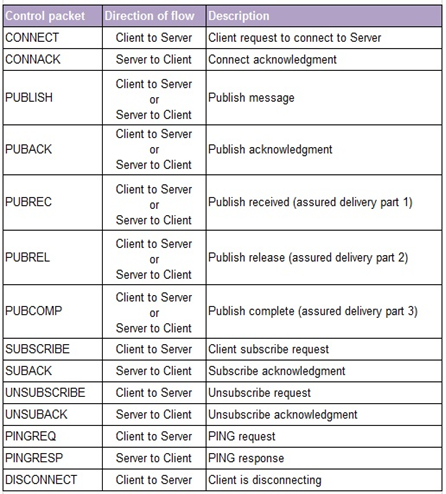
\includegraphics[width=1.0\columnwidth]{images/MQTT.png}
\caption{MQTT Publish Subscribe Architecture}




\end{figure}



\section{Conclusion}
There is tremendous application prospects of using MQTT protocol in big data and edge computing. Edge computing, being a new  development in data analytics,  has enormous use as the volume of data is increasing at such an unimaginable rate. MQTT is simple to use and configure, it is a great platform for edge computing. All the commercial, industrial, service and development sectors are moving towards modernization with regard to using newer technology. Newer technologies are being developed in some way as a medium of making business, industries health care, military and other sectors efficient. Iots newer applications demand edge computing for quicker data analysis and MQTT as a simple to use protocol.  


\begin{acks}

  The author would like to thank Dr. Gregor von Laszewski for his
  support and suggestions to write this paper.

\end{acks}

\bibliographystyle{ACM-Reference-Format}
\bibliography{report} 



\end{document}
